% 2008 年福建卷理科第 21 题：椭圆 x²/a²+y²/b²=1（a>b>0），焦点 F(1,0)，O 为原点；
%   过 F 的直线 l 交椭圆于 A、B。
% 来源 PDF：gaokaomath-src/普通高考/2008/2008福建理.pdf
% SHA-256：516e8ac8e113868afa9bc4af4724c3b43f22a1f7fecc830a7f3400b8d973d452
% 原页：2008福建理.pdf 第 2 页（A3 三栏）第 2 栏，书页码 442。
% 重绘依据：按原页画椭圆与 x/y 轴，F 在 x 轴正半轴上；过 F 的直线 l 与椭圆交于
%   第一象限的 A 与第三象限的 B。取图示椭圆 x 半径 2.6、y 半径 1.75，A、B 取在椭圆上
%   且与 F 共线（A≈(1.99,1.13)、B≈(−0.51,−1.72)），l 在两端各延长一小段。
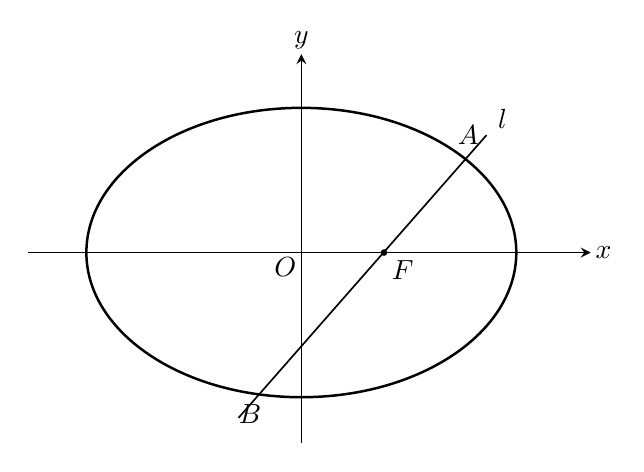
\begin{tikzpicture}[x=1.05cm, y=1.05cm, semithick, every node/.style={inner sep=1.5pt}]
  \draw[->,>=stealth] (-3.3,0) -- (3.5,0) node[right] {$x$};
  \draw[->,>=stealth] (0,-2.3) -- (0,2.4) node[above] {$y$};
  \node[below left] at (0,0) {$O$};

  \draw[line width=0.9pt] (0,0) ellipse [x radius=2.6, y radius=1.75];

  \coordinate (F) at (1,0);
  \coordinate (A) at (1.99,1.13);
  \coordinate (B) at (-0.51,-1.72);

  \draw (-0.76,-2.00) -- (2.24,1.42);
  \node[right] at (2.32,1.62) {$l$};

  \fill (F) circle (1.2pt);
  \node[below right=1pt] at (F) {$F$};
  \node at (2.02,1.42) {$A$};
  \node at (-0.62,-1.95) {$B$};
\end{tikzpicture}
